\begin{frame}
  \frametitle{Definición Procesos}
  \begin{itemize}
	  \item Programa en ejecución
	  \item Los conceptos de tarea, job y proceso hacen referencia a lo mismo
	  \item Según su historial de ejecución, los podemos clasificar en:
	  \begin{itemize}
	  	\item CPU Bound (ligados a la CPU)
	  	\item I/O Bound (ligados a entrada/salida)
	  \end{itemize}
  \end{itemize}
\end{frame}

\begin{frame}
  \frametitle{Definición Procesos (cont.)}
  \begin{itemize}
	  \item Programa
	  \begin{itemize}
	  	\item Es estático
	  	\item No tiene program cunter
	  	\item Existe desde que se edita hasta que se borra
	  \end{itemize}
	  \begin{figure}
		    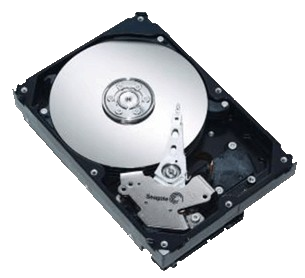
\includegraphics[scale=0.1]{images/program.png}
	  \end{figure}
	  \item Proceso
	  \begin{itemize}
	  	\item Es dinámico
	  	\item Tiene program counter
	  	\item Su ciclo de vida comprende desde que se lo ejecuta hasta que termina
	  \end{itemize}
	  \begin{figure}			
			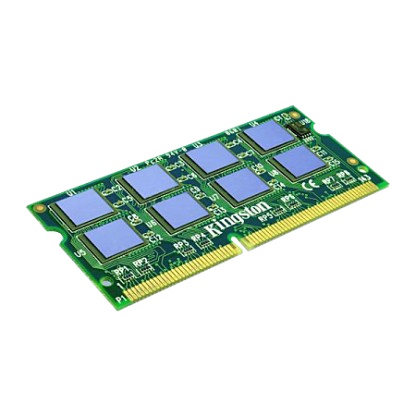
\includegraphics[scale=0.1]{images/process.png}
	  \end{figure}	  
  \end{itemize}
\end{frame}

\begin{frame}
  \frametitle{Procesos - \textbf{PCB}}
  \begin{itemize}
	  \item Una por proceso
	  \item Contiene información del proceso
	  \item Es lo primero que se crea cuando se realiza un \textit{fork} y lo último que se desaloca cuando termina
	  \begin{figure}
			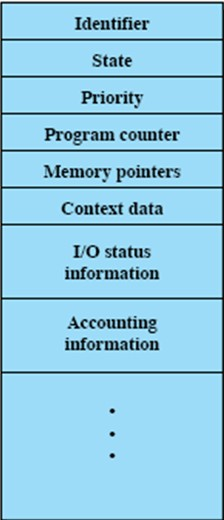
\includegraphics[scale=0.2]{images/pcb.png}
	  \end{figure}	  
  \end{itemize}
\end{frame}

\begin{frame}
  \frametitle{Procesos - \textbf{Estados}}
  \begin{figure}
		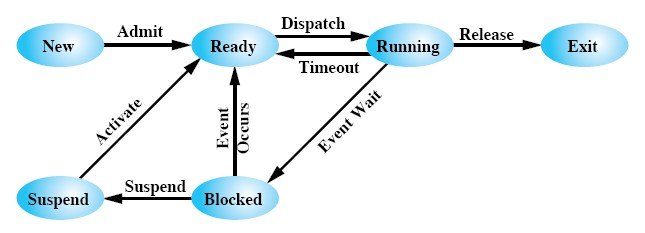
\includegraphics[scale=0.5]{images/statesProcess.png}
  \end{figure}
\end{frame}

\begin{frame}
  \frametitle{Planificadores - \textbf{Objetivo}}
  \begin{itemize}
	  \item Es la clave de la multiprogramación
	  \item Esta diseñado de manera apropiada para cumplir las metas de:
	  \begin{itemize}
	  	\item Menor Tiempo de Respuesta
	  	\item Mayor rendimiento
	  	\item Uso eficiente del procesador
	  \end{itemize}
  \end{itemize}
\end{frame}

\begin{frame}
  \frametitle{Planificadores - \textbf{Tipos}}
  \begin{itemize}
		\item \textbf{Long term scheduler}: admite nuevos procesos a memoria (controla el grado de multirpogramación)
		\item \textbf{Medium term scheduler}: realiza el \emph{swapping} (intercambio) entre el disco y la memoria cuando el SO lo determina (puede disminuir el grado de multiprogramación)
		\item \textbf{Short term scheduler}: determina que proceso pasará a ejecutarse
  \end{itemize}
\end{frame}

\begin{frame}
  \frametitle{Planificadores y Estados}
  \begin{figure}
    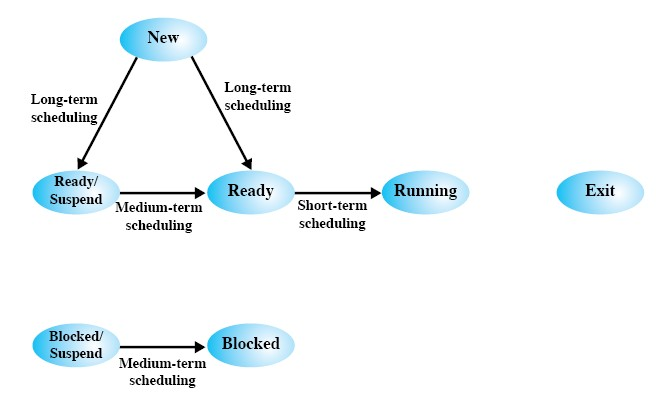
\includegraphics[scale=0.4]{images/statesSchedulers.png}
  \end{figure}
\end{frame}

\begin{frame}
  \frametitle{Planificadores y Colas}
  \begin{figure}
    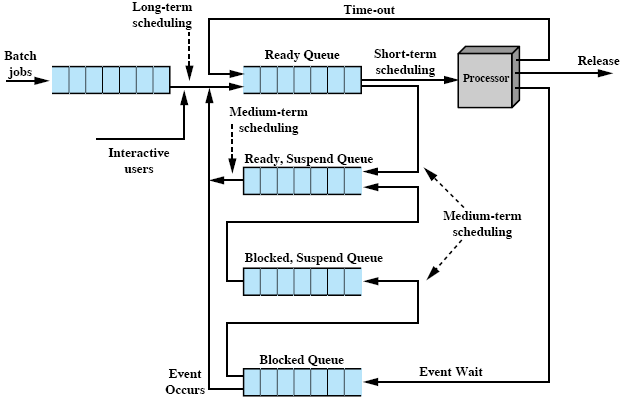
\includegraphics[scale=0.4]{images/queuesSchedulers.png}
  \end{figure}
\end{frame}

\begin{frame}
  \frametitle{Tiempos de los procesos}
  \begin{itemize}
		\item \textbf{Retorno}: tiempo que transcurre entre que el proceso llega al sistema hasta que completa su ejecución
		\item \textbf{Espera}: tiempo que el proceso se encuentra en el sistema esperando, es decir el tiempo que pasa sin ejecutarse (\textbf{TR - Tcpu})
		\item \textbf{Promedios}: tiempos promedio de los anteriores
  \end{itemize}
\end{frame}

\begin{frame}
  \frametitle{Apropiación vs No Apropiación}
  \begin{itemize}
		\item \textbf{Nonpreemptive}: una vez que un proceso esta en estado de ejecución, continua hasta que termina o se bloquea por algún evento (e.j. I/O)
		\item \textbf{Preemptive}: el proceso en ejecución puede ser interrumpido y llevado a la cola de listos:
		\begin{itemize}
			\item Mayor overhead pero mejor servicio
			\item Un proceso no monopoliza el procesador
		\end{itemize}
  \end{itemize}
\end{frame}

\begin{frame}
  \frametitle{Algoritmo \textbf{FIFO}}
  \begin{itemize}
		\item Firs come first served
		\item Cuando hay que elegir un proceso para ejecutar, se selecciona el mas viejo
		\item No favorece a ningún tipo de procesos, pero en principio prodíamos decir que los \textit{CPU Bound} terminan al comenzar su primer ráfaga, mientras que los \textit{I/O Bound} no
  \end{itemize}
\end{frame}

\begin{frame}[fragile]
  \frametitle{Algoritmo \textbf{FIFO} (cont.)}
  \begin{table}
      \centering
      \resizebox{15pc}{!}{
	  \begin{tabular}{| c | c | c | c |}
	      \hline
	      \bf Job & \bf Llegada & \bf CPU & \bf Prioridad \\
	      \hline
	      1 & 0 & 9 & 3 \\
	      \hline
	      2 & 1 & 5 & 2 \\
	      \hline
	      3 & 2 & 3 & 1 \\
	      \hline
	      4 & 3 & 7 & 2 \\
	      \hline
	  \end{tabular}
      }
  \end{table}  
  \begin{lstlisting}
#Ejemplo 1
TAREA ''1'' PRIORIDAD=3
[CPU,9]
TAREA ''2'' PRIORIDAD=2
[CPU,5]
TAREA ''3'' PRIORIDAD=1
[CPU,3]
TAREA ''4'' PRIORIDAD=2
[CPU,7]  
  \end{lstlisting}  
  \hspace{35pt} \textcolor{orange}{¿Cuáles serían los tiempos de retorno y espera?}
\end{frame}

\begin{frame}
  \frametitle{Algoritmo \textbf{SJF}}
  \begin{itemize}
  		\item Shortest Job First
		\item Política \textit{nonpreemptive} que selecciona el proceso con la ráfaga más corto
		\item Calculo basado en la ejecución previa
		\item Procesos cortos se colocan delante de procesos largos
		\item Los procesos largos pueden sufrir \textit{starvation} (inanición)
  		\pause
  		\item \textcolor{orange}{Veamos el ejemplo anterior}	
  \end{itemize}
\end{frame}

\begin{frame}
  \frametitle{Algoritmo \textbf{RR}}
  \begin{itemize}
  		\item Round Robin
		\item Politica basada en un reloj
		\item \textbf{Quantum (Q)}: medida que determina cuanto tiempo podrá usar el procesador cada preceso:
		\begin{itemize}
			\item Pequeño: overhead de \textit{context switch}
			\item Grande: ¿pensar?
		\end{itemize}
		\item Cuando un proceso es expulsado de la \textit{CPU} es colocado al final de la \textit{Ready Queue} y se selecciona otro (\textit{FIFO circular})
  \end{itemize}
\end{frame}

\begin{frame}
  \frametitle{Algoritmo \textbf{RR} (cont.)}
  \begin{itemize}
  		\item Existe un ``contador'' que indica las unidades de CPU en las que el proceso se ejecuto. Cuando el mismo llega a 0 el proceso es expulsado
		\item El ``contador'' puede ser:
		\begin{itemize}
			\item Global
			\item Local $\rightarrow$ \textit{PCB}
		\end{itemize}  		
		\item Existen dos variantes con respecto al valor inicial del ``contador'' cuando un proceso es asignado a la CPU:
		\begin{itemize}
			\item \textbf{Timer Variable}
			\item \textbf{Timer Fijo}
		\end{itemize}
  \end{itemize}
\end{frame}

\begin{frame}
  \frametitle{Algoritmo \textbf{RR - Timer Variable}}
  \begin{itemize}
  		\item El ``contador'' se inicializa en Q (contador := Q) cada vez que un proceso es asignado a la \emph{CPU}
		\item Es el más utilizado
		\item Utilizado por el simulador
		\pause
		\item \textcolor{orange}{Veamos el ejemplo 1 nuevmanete}
  \end{itemize}
\end{frame}

\begin{frame}
  \frametitle{Algoritmo \textbf{RR - Timer Fijo}}
  \begin{itemize}
  		\item El ``contador'' se inicializa en Q cuando su valor es cero
  		\begin{itemize}
  			\item if (contador == 0) contador = Q;
  		\end{itemize}
		\item Se puede ver como un valor de Q compartido entre los procesos
  \end{itemize}
\end{frame}

\begin{frame}
  \frametitle{Algoritmo \textbf{RR} (cont.)}
	\begin{figure}
	    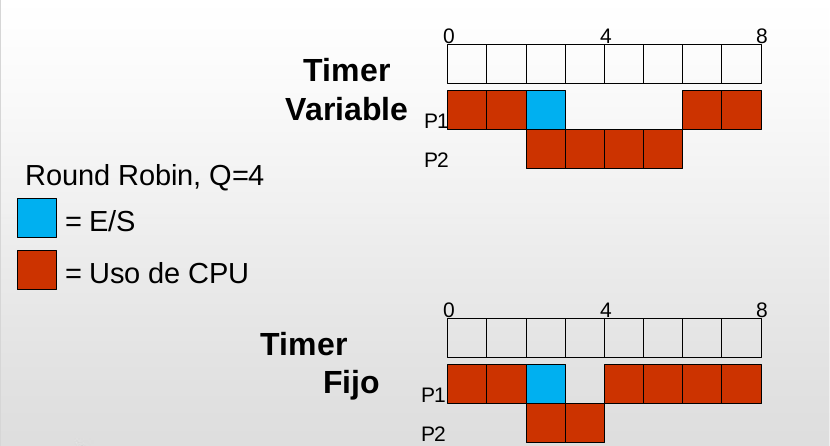
\includegraphics[scale=0.4]{images/ejemploRR.png}
	\end{figure}
\end{frame}

\begin{frame}
  \frametitle{Algoritmo con \textbf{Uso de Prioridades}}
  \begin{itemize}
  		\item Cada proceso tiene un valor que representa su prioridad $\rightarrow$ menor valor, mayor prioridad
		\item Se selecciona el proceso de mayor prioridad de los que se encuentran ela \emph{Ready Queue}
		\item Existe una \emph{Ready Queue} por cada nivel de prioridad
		\item Procesos de baja prioridad pueden sufrir \emph{starvation} (inanición)
		\begin{itemize}
			\item Solución: permitir a un proceso cambiar su prioridad durante su ciclo de vida $\rightarrow$ \textbf{Aging}
		\end{itemize}
		\item Puede ser un algoritmo \textbf{preemptive} o no
		\pause
		\item \textcolor{orange}{Veamos el ejemplo 1 nuevamente}
  \end{itemize}
\end{frame}

\begin{frame}
  \frametitle{Algoritmo con Uso de Prioridades (cont.)}
	\begin{figure}
	    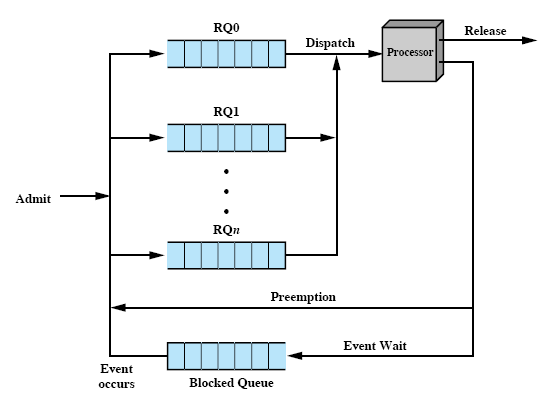
\includegraphics[scale=0.4]{images/priorities.png}
	\end{figure}
\end{frame}

\begin{frame}
  \frametitle{Algoritmo \textbf{SRTF}}
  \begin{itemize}
  		\item Shortest Remaining Time First  		
		\item Versión \emph{preemptive} de \textit{SJF}
		\item Selecciona el proceso al cual le resta menos tiempo de ejecución en su siguiente ráfaga.
		\item ¿A qué tipos de procesos favorece?
		\pause
		\textbf{$\rightarrow$ I/O Bound}
		\pause
		\item \textcolor{orange}{Veamos el ejemplo 1 nuevamente}
  \end{itemize}
\end{frame}

\begin{frame}
  \frametitle{Algoritmos de planificación - CPU + I/O}
  \begin{itemize}
  		\item Ciclo de vida de un proceso: uso de CPU + operaciones de I/O
		\item Cada dispositivo tiene su cola de procesos en espera $\rightarrow$ un scheduler por cada cola
		\item Se considera I/O independiente de la CPU (DMA, PCI, etc.) $\rightarrow$ uso de CPU y operaciones de I/O en simultaneo
  \end{itemize}
\end{frame}

\begin{frame}
  \frametitle{Algoritmos de planificación - Criterios de desempate}
  \begin{itemize}
  		\item Orden de aplicación:
  		\begin{itemize}
  			\item Orden de llegada de los procesos
  			\item \textbf{PID} de los procesos
  		\end{itemize}

		\item Siempre se mantiene la misma politica
  \end{itemize}
\end{frame}

\begin{frame}[fragile]
  \frametitle{Algoritmos de planificación - Un recurso por proceso}
  \begin{table}
      \centering
      \resizebox{15pc}{!}{
		  \begin{tabular}{| c | c | c | c |}
		      \hline
		      \bf Job & \bf Llegada & \bf CPU & \bf E/S (rec., inst., dur.) \\
		      \hline
		      1 & 0 & 5 & (R1, 3, 2) \\
		      \hline
		      2 & 1 & 4 & (R2, 2, 2) \\
		      \hline
		      3 & 2 & 3 & (R3, 2, 3) \\
		      \hline
		  \end{tabular}
      }
  \end{table}
  \begin{lstlisting}
#Ejemplo 2
RECURSO ''R1''
RECURSO ''R2''
RECURSO ''R3''
TAREA ''1'' INICIO=0
[CPU,3] [1,2] [CPU,2]
TAREA ''2'' INICIO=1
[CPU,2] [2,2] [CPU,2]
TAREA ''3'' INICIO=2
[CPU,2] [3,3] [CPU,1]
  \end{lstlisting}
\end{frame}

\begin{frame}[fragile]
  \frametitle{Algoritmos de planificación - Recurso compartido}
  \begin{table}
      \centering
      \resizebox{15pc}{!}{
		  \begin{tabular}{| c | c | c | c |}
		      \hline
		      \bf Job & \bf Llegada & \bf CPU & \bf E/S (rec., inst., dur.) \\
		      \hline
		      1 & 0 & 5 & (R1, 3, 3) \\
		      \hline
		      2 & 1 & 4 & (R1, 1, 2) \\
		      \hline
		      3 & 2 & 3 & (R2, 2, 3) \\
		      \hline
		  \end{tabular}
      }
  \end{table}
  \begin{lstlisting}
#Ejemplo 3
RECURSO ''R1''
RECURSO ''R1''
TAREA ''1'' INICIO=0
[CPU,3] [1,3] [CPU,2]
TAREA ''2'' INICIO=1
[CPU,1] [1,2] [CPU,3]
TAREA ''3'' INICIO=2
[CPU,2] [2,3] [CPU,1]
  \end{lstlisting}
\end{frame}

\begin{frame}
  \frametitle{Esquema \textbf{Colas Multinivel}}
  \begin{itemize}
  		\item Scheduler actuales $\rightarrow$ combinación de algoritmos vistos
		\item La \emph{ready queue} es dividida en varias colas (similar a prioridades)		
		\item Los procesos se colocan en las colas según una clasificación que realise el sistema operativo
		\item Cada cola posee su propio algoritmo de planificación $\rightarrow$ \textbf{planificador horizontal}
		\item A su vez existe un algoritmo que planifica las colas $\rightarrow$ \textbf{planificador vertical}
		\item Retroalimentacion $\rightarrow$ un proceso puede cambiar de una cola a la otra
  \end{itemize}
\end{frame}

\begin{frame}
  \frametitle{Esquema \textbf{Colas Multinivel} (ejemplo 1)}
	\begin{figure}
	    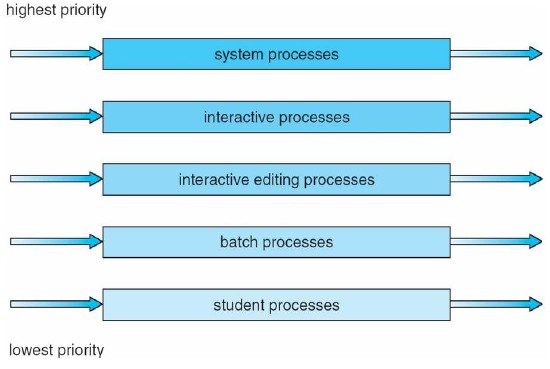
\includegraphics[scale=0.4]{images/multilevelSchemaExample1.png}
	\end{figure}
\end{frame}

\begin{frame}
  \frametitle{Esquema \textbf{Colas Multinivel} (ejemplo 2)}
  \begin{itemize}
  		\item El sistema consta de tres colas:
  		\begin{itemize}
  			\item Q0: se planifica con \emph{RR, q=8}
  			\item Q1: se planifica con \emph{RR, q=16}
  			\item Q2: se planifica con \emph{FCFS}
  		\end{itemize}
  		\item Para la planificacion se utilizan los siguientes criterios:
  		\begin{itemize}
  			\item Los procesos ingresan en la \emph{Q0}. Si no se utilizan los 8 cuantos el job es movido a la cola \emph{Q1}
  			\item Para la cola \emph{Q1}, el comportamiento es similar a \emph{Q0}. Si un proceso no finaliza su ráfaga de 16 instantes, es movido a la cola \emph{Q2}
  		\end{itemize}
  \end{itemize}
\end{frame}

\begin{frame}
  \frametitle{Esquema \textbf{Colas Multinivel} (ejemplo 2 cont.)}
	\begin{figure}
    	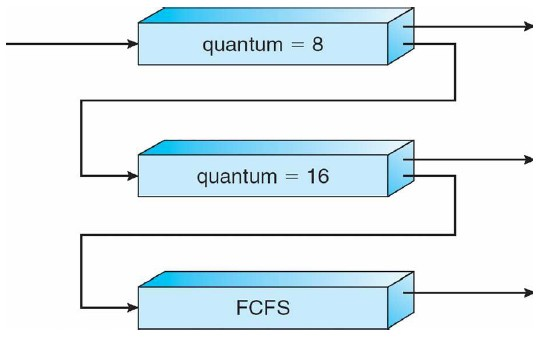
\includegraphics[scale=0.4]{images/multilevelSchemaExample2.png}
	\end{figure}
	\begin{itemize}
		\pause
		\item \textcolor{orange}{¿A qué procesos beneficia el algoritmo?}
		\pause
		$\rightarrow$ \textbf{CPU Bound}
	\pause  			
		\item \textcolor{orange}{¿Puede ocurrir inanición?}
	\pause
		$\rightarrow$ Si, con los procesos ligados a \emph{E/S} si siempre llegan procesos ligados a \emph{CPU}
	\end{itemize}
\end{frame}

\begin{frame}
  \frametitle{Planificación con múltiples procesadores}
	\begin{itemize}
		\item La planificación de CPU es más compleja cuando hay múltiples CPUs	
		\item Este enfoque fue implementado inicialmente en \textit{Mainframes} y luego en \textit{PC}
		\item La carga se divide entre distintas CPUs, logrando capacidades de procesamiento mayores
		\item Si un procesador falla, el resto toma el control
	\end{itemize}
\end{frame}

\begin{frame}
  \frametitle{Planificación con múltiples procesadores: \textbf{Criterios}}
	\begin{itemize}
		\item \textbf{Planificación temporal} $\rightarrow$ que proceso ejecutar
		\item \textbf{Planificación espacial} $\rightarrow$ en que procesador ejecutar el proceso:		
		\begin{itemize}
			\item \textbf{Huella}: estado que el proceso va dejando en la cache de un procesador
			\item \textbf{Afinidad}: preferencia de un proceso para ejecutar en un procesador 
		\end{itemize}
		\item La asignación de procesos a un procesador puede ser:
		\begin{itemize}
			\item \textbf{Estática}: existe una afinidad de un proceso a una CPU
			\item \textbf{Dinámica}: la carga se comparte $\rightarrow$ balanceo de carga
		\end{itemize}
		\item La política puede ser:
		\begin{itemize}
			\item \textbf{Tiempo compartido}: se puede cosiderar una \emph{cola global} o una \emph{cola local} a cada procesado
			\item \textbf{Espacio compartido}:
			\begin{itemize}
				\item \textbf{Grupos} (\emph{threads})
				\item \textbf{Particiones}
			\end{itemize}
		\end{itemize}		
	\end{itemize}
\end{frame}

\begin{frame}
  \frametitle{Planificación con múltiples procesadores (cont.)}
	\begin{itemize}		
		\item \emph{Clasificaciones}:
		\begin{itemize}
			\item \textbf{Procesadores homogéneos}: todas las CPUs son iguales. No existen ventajas físicas sobre el resto
			\item \textbf{Procesadores heterogéneos}: cada procesador tiene su propia cola y algoritmo de planificación
		\end{itemize}
		\item \emph{Otra clasificación}:
		\begin{itemize}
			\item \textbf{Procesadores débilmente acoplados}: cada CPU tiene su propia memoria principal y canales
			\item \textbf{Procesadores fuertenemente acoplados}: comparten memoria y canales
			\item \textbf{Procesadores especializados}: uno o más procesadores principales de uso general y uno o más procesadores de uso específico
		\end{itemize}		
	\end{itemize}
\end{frame}